%!TEX root = thesis.tex
\chapter{Pipeline Design and Implementation}
\label{sec:implementation}

This chapter describes the design and implementation of the prototype data filtering pipelines to be built for testing
and evaluating our candidate data stream processing system (DSPS) technologies. This will be performed with the intention
of arriving at a recommendation system for the case study of the Monash University Institute of Railway Technology (IRT)
project. Each of the candidate DSPS technologies have been detailed in-depth in previous chapters, and all exhibit the capabilities
needed to implement the intended prototype pipelines.

This chapter will first go into the design of the data filtering pipeline, in~\sectref{sub:pipeline_design}, before
detailing the testing environment which was used to implement and test each pipeline, in~\sectref{sub:testing_environment_details}.
In~\sectref{sub:implementation_of_pipelines_in_dsps_technol}, the implementation of the prototype pipelines will be
detailed for each of the candidate DSPS technologies, as well as looking at the programming possibilities afforded by
each technology. Finally, the chapter will be concluded in~\sectref{sub:implement_conclusion}.


\section{Data Filtering Pipeline Design} % (fold)
\label{sub:pipeline_design}

The overall design of the data filtering pipeline will be designed in such a way that readings from sensors can be fed
into the pipeline, processed in some specified manner, then output for further use, including storage for batch processing,
or discarded in the case of noisy data. Thinking of the pipeline in such a way, we can decompose the design into three main
components:

\begin{enumerate}
  \item Sensor data input component
  \item Sensor data processing component
  \item Results output component
\end{enumerate}

Each component would also need to connect somehow to form the entire pipeline design. The components are listed
in order of their precedence of their role in the pipeline. Hence, the first component's output would be the input to
the second component, of which the output would be the input to the third component. This creates the dataflow behaviour
exhibited in pipelines. This basic design that we have so far is illustrated in~\figref{fig:pipeline_simple}.

\begin{figure}[ht]
  \centering
  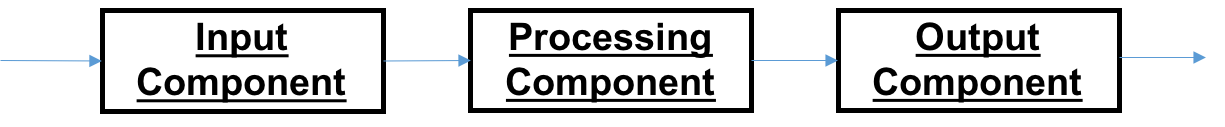
\includegraphics[width=0.8\textwidth]{includes/figures/fig_pipeline_simple}
  \caption{A simplistic overview of our pipeline design. Note the dataflow behaviour exhibited with each component's output
  being an input of the following component.}
  \label{fig:pipeline_simple}
\end{figure}

We now have a simple design of the pipeline, however we are left with the questions of the output of the \textbf{Output Component},
the input of the \textbf{Input Component}, and the contents of each component.

The output of the \textbf{Output Component}
will simply be whatever extensions are needed to be made to the pipeline. Hence, rather than acting a sink, this component
will be an abstract interface which any extension needed will be able to adhere to extend the pipeline. Designing the pipeline
in this manner directly addresses our third research question touched upon in Chapter 1, in~\sectref{sub:research_questions}.
This allows the output data to be dealt with in any manner required by the IRT team, whether it be stored for later
batch processing, or forwarded on for further realtime processing.

The input of the \textbf{Input Component} will be the data read from the sensors to which the pipeline is connected to.
The sensors generally would not be directly connected to the pipeline, so we could have another abstract interface here
that any sensor connects to, then the interface sends the data to the actual component. This allows data to be fed into
the pipeline from any type of sensor that is able to adhere to the interface.

The contents of each component is a larger task. The \textbf{Processing Component} will be made up
of an arbitrary number of tasks, each of which are tasked to process the data in some manner before forwarding it onto whatever
the next specified task is. This, in itself, acts as a mini-pipeline where the core of processing will be done. Here
we will say that the \textbf{Processing Component} consists of $n$ sequential processing tasks. For the \textbf{Input Component},
the contents will consist of a task-like component tasked with passing data onto the processing tasks which make up the
\textbf{Processing Component}. The contents of the
\textbf{Output Component} will be as described previously: an abstract interface allowing for the extension of the pipeline.

This leaves us with a final pipeline design as illustrated in~\figref{fig:pipeline_whole}.

\begin{figure}[ht]
  \centering
  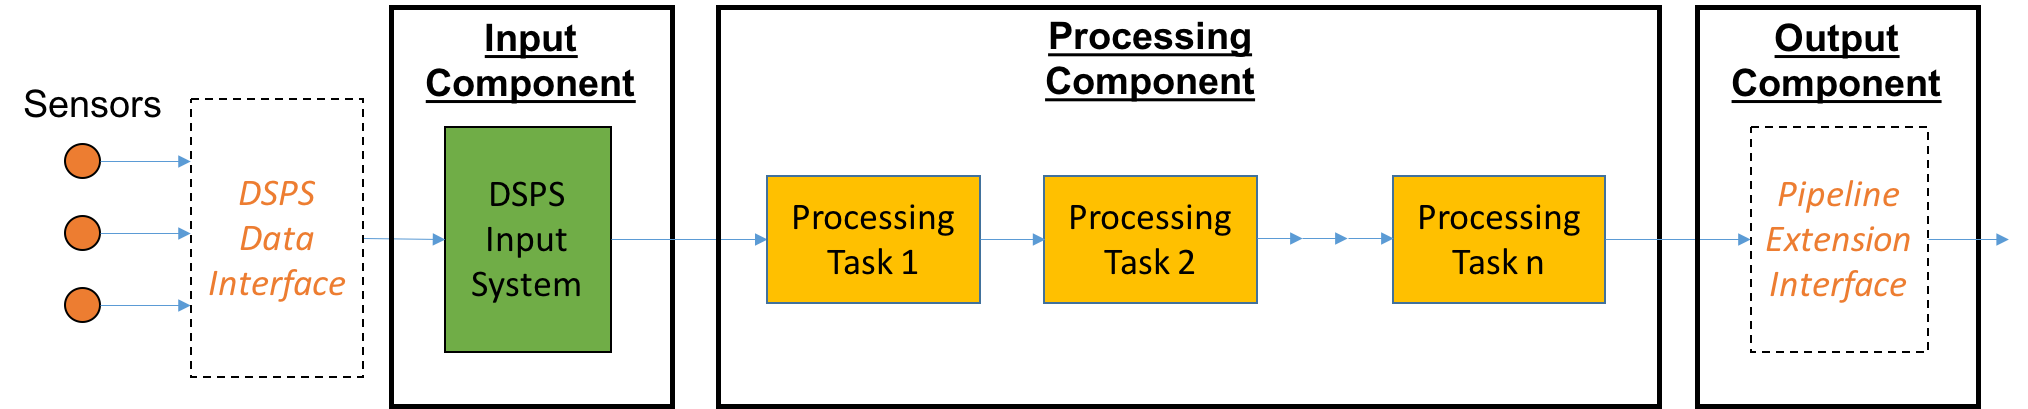
\includegraphics[width=1\textwidth]{includes/figures/fig_pipeline_whole}
  \caption{A complete overview of our pipeline design.}
  \label{fig:pipeline_whole}
\end{figure}

Note that this diagram illustrates an overall abstract pipeline design. However, for implementation of the pipeline which
will be used in the evaluation parts of the project, we need to implement concrete components for testing. In this project,
we do not have access to any sensors, or any such hardware, for sending readings to the pipeline for processing. Hence, for evaluation
we have had to simulate the sensor component of the overall pipeline design in some way. Note that this does not affect
the pipeline in any way, since the actual sensor hardware part of the design is abstracted away from the software pipeline
itself. The function of the sensors is to send data to the pipeline at any arbitrarily specified interval through use of the
DSPS Data Interface.
To simulate this functionality multiple methods exist. The most basic of such is arguably reading data from a file
and placing that onto a stream for the pipeline to process. However, this very much mimics batch processing methods, and
hence is not ideal for simulating realtime data. Furthermore, placing data from a file onto the pipeline does not accurately
reflect the client-server networking functionality that will exist in a real sensor-pipeline connection.

A better way to simulate this sensor-pipeline realtime data connection is to develop a data entry interface to the pipeline upon which data can be sent to
at any time. This data entry interface can then be used to simulate arbitrarily specified intervals upon which data can be sent,
thus mimicking the functionality of a sensor. To do this while still adhering to the client-server connection design,
we can use a socket connection, allowing data to be sent over a specified port to be placed upon the pipeline. Each
candidate DSPS technology either has native support for server socket connections, given their commonplace as mediums upon
which data can be sent over, or support from the programming language standard libraries used to implement realtime processing logic.

Hence, the \textbf{Input Component} will be implemented as a server socket connection,
and the \textbf{Processing Component} as a filtering task. Speed sensor readings will be passed in along the socket connection
using a tool allowing interface to network ports, such as \texttt{netcat}\footnote{http://netcat.sourceforge.net/}, and filtered to make sure they are valid
speed values, between the limits of 0 and 90. Any speeds
outside of these limits can safely be deemed to be either bad, or noisy, sensor readings. This results in a concrete design as shown
in~\figref{fig:pipeline_concrete}.

\begin{figure}[ht]
  \centering
  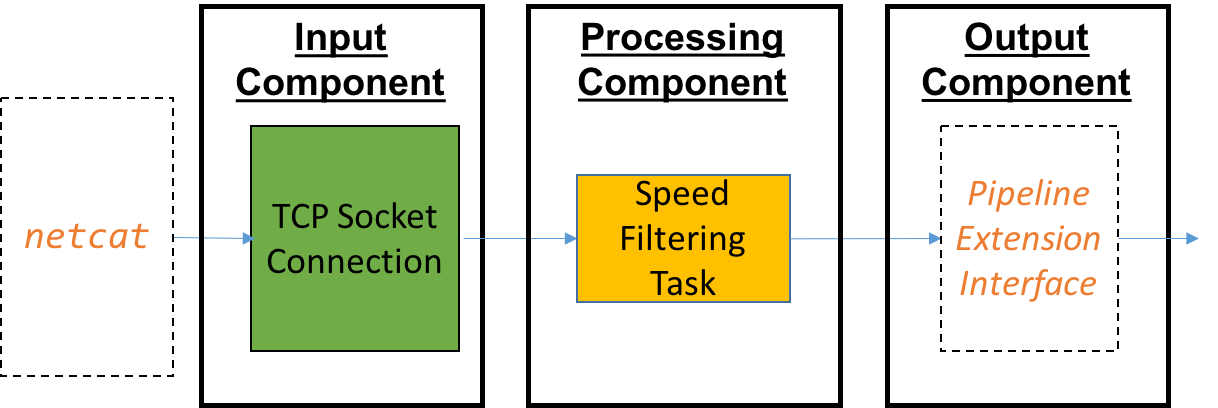
\includegraphics[width=0.8\textwidth]{includes/figures/fig_pipeline_concrete}
  \caption{A concrete implementation of our pipeline design.}
  \label{fig:pipeline_concrete}
\end{figure}

% subsection pipeline_design (end)


\section{Testing Environment Details} % (fold)
\label{sub:testing_environment_details}

\subsection{Details on Host System} % (fold)
\label{ssub:host_system}

The testing environment on which the prototype pipelines were implemented using each of the candidate DSPS technologies
is the same National eResearch Collaboration Tools and Resources (NeCTAR) cloud computing environment touched upon
briefly in Chapter 1. This cloud service platform is provided as an initiative by the Australian Government for researchers
that require the infrastructure\footnote{https://www.nectar.org.au/about-nectar}.

Our environment consists of a single NeCTAR cloud instance of which the details are specified in~\tabref{tab:control}.

\begin{table}[ht]
\caption{Control system used for testing pipelines.}
\label{tab:control}
\centering
\begin{tabular}{ll}
\textbf{Distribution}         & Ubuntu GNU/Linux 14.04.2 LTS \\
\textbf{Kernel}               & Linux 3.13.0-36-generic    \\
\textbf{Architecture}         & x86\_64                    \\
\textbf{Virtual CPUs}         & 16                         \\
\textbf{Available RAM}        & 64 GB                      \\
\textbf{Available Disk Space} & 490 GB
\end{tabular}
\end{table}

The NeCTAR cloud instance utilises a single node upon which all processing is performed. In a real deployment, it is
common to use a full cluster upon which the pipeline would be deployed, where processing is shared and distributed between nodes. Due to
limited testing resources, all testing
has been performed on a single node cluster, however this remains a constant feature between all implementation and tests
performed in the project. Furthermore, the pipelines built upon
each of the candidate DSPS technologies are freely configurable to be deployed to run on arbitrarily sized clusters without
requiring changes to the underlying source code.

% subsubsection host_system (end)


\subsection{Details on Data Stream Processing System Technologies} % (fold)
\label{sub:setting_up_of_dsps_technologies}

The DSPS technologies that have been chosen to be focused on in this sub-project include the following:

\begin{itemize}
  \item Samza
  \item Storm
  \item Spark Streaming
\end{itemize}

Literature concerning these DSPS technologies have been covered in~\sectref{sub:realtime_data_processing}, however
we will look into more depth into the systems regarding their usage from the programmer's point-of-view. Note that
in the previous chapter, a further DSPS technology, S4, was covered, however due to its noted decline in usage and
development in the chapter, it has been decided to omit the use of the technology from this project.

Version 0.9.0 of Samza was used for implementation of the prototype pipeline in Samza. At the time of implementation,
this was the major stable version of Samza, accepted as a top-level Apache project. Java, the only official programming
language supported by the Samza project, was used, using JDK 1.8.0 as the target implementation.

Version 0.9.4 of Storm was used for implementation of the prototype pipeline in Storm. As with Samza, this was also the
major stable version of Storm available. Java 8 was used as the implementation language, also compiling for the JDK 1.8.0.

Version 1.3.0 of Spark and the Spark Streaming extension were used for the Spark Streaming implementations. Prototype pipelines were
implemented in both Scala 2.9.2, targeting the JDK 1.8.0, and Python 2.7, which is made possible through the relatively new (as of Spark 1.2.0)
PySpark subsystem. Implementations for the Spark Streaming pipeline were built targeting both Spark JVM and PySpark due
to numerous undocumented claims that performance differs on both Spark implementations. These claims are addressed further
in the following chapter.

The specific JDK implementation for all tests was the Intel 64-bit OpenJDK 1.8.0 release 45 built and packaged for the GNU/Linux
distribution of Ubuntu 14.04.2 LTS.

% subsubsection setting_up_of_dsps_technologies (end)

% subsection testing_environment_details (end)


\section{Implementation of Pipelines in Data Stream Processing System Technologies} % (fold)
\label{sub:implementation_of_pipelines_in_dsps_technol}

Here, we will look at how the each of the candidate DSPS technologies were used for implementation in relation to our testing
pipeline design. We will look at the possibilities each technology affords in terms of programmability, and then what was
required to be implemented for our testing and evaluation to arrive at a DSPS recommendation.

For each DSPS technology, we will look at what was needed to be implemented for the following components from our design:

\begin{itemize}
  \item Input component
  \item Processing component
  \item Output component
\end{itemize}

\subsection{Samza} % (fold)
\label{ssub:impl_samza}

Samza defines itself as a realtime data processing system, which allows the processing of streams made up of immutable
messages of similar type or category. Streams in Samza exist independently of other concepts, allowing themselves to be
\textit{consumed} from or \textit{produced} to by various supported systems. The concepts of consuming and producing refer
to the actions of getting data from a stream and placing data onto a stream, respectively. Samza defines the systems that can be used
for consuming and producing to streams to be any piece of software that implements the stream abstraction. For example,
Kafka, a popular distributed messaging queueing system, is often used to consume and produce to Samza streams. Systems such as these can be
``plugged'' into a Samza project to work with the same streams which native Samza applications are written to work with~\cite{Samza:doc}.

For a Samza programmer, the most important concepts of the overall Samza project to understand are the concepts of the
\textbf{system} and \textbf{task}. In a Samza project, a system exists to produce a particular stream from some source
of data which then can
be processed by a task which consumes it. A task will always perform some processing before producing the results as output to another stream. Systems and tasks
can then be arranged in a pipeline-like structure allowing a specified type of processing on the messages which travel
on those streams. Hence, it is easy to think of a system as the source of data for an overall Samza project. A very
simple example of such a Samza project is shown in~\figref{fig:samza_overview}.

\begin{figure}[ht]
  \centering
  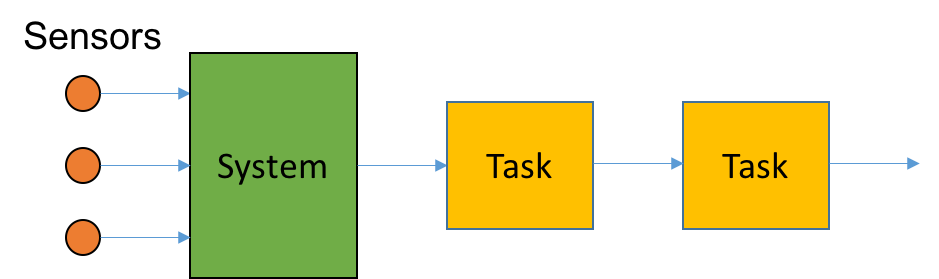
\includegraphics[width=0.8\textwidth]{includes/figures/fig_samza_overview}
  \caption{A simple Samza pipeline showing the roles of the system (handling input data), task (handling data processing), and stream concepts. Streams are represented
  as arrows.}
  \label{fig:samza_overview}
\end{figure}

\subsubsection{Programming Overview}

When programming a Samza project, interfaces exist for both the system and task concepts through the \path{org.apache.samza.system.SystemConsumer}
and \path{org.apache.samza.task.StreamTask} Java interfaces~\cite{Samza:doc}. Default systems exist in the Samza project, and may be
used to produce streams which can then be processed by an implemented \texttt{StreamTask}.

The \texttt{StreamTask} interface is arguably the main interface in which the most important processing will be done in
a Samza project. It requires implementing a single method, \texttt{process}, which passes in an immutable message from the stream
on which the task is configured to consume. These messages are then processed as specified by the programmer, before the
result of the processing is wrapped in a message envelope and produced to a stream, also specified by the programmer~\cite{Samza:doc}.

The streams on which \texttt{StreamTask} implementations consume are specified in a task specific configuration file,
independent to that of the implementation source code. These configuration files offer a range of parameters for the
execution of tasks, each of which are documented\footnote{https://samza.apache.org/learn/documentation/0.9/jobs/configuration-table.html},
however can result in quite verbose and hard to understand configuration files. For each task configuration, a system
needs to be defined that produces to the stream that the task consumes from. These can either be a self-implemented
system, or an existing pluggable system, such as Kafka~\cite{Samza:doc}.

For self-implementation of systems, the \texttt{SystemConsumer} interface requires much more understanding and effort to
implement than that of the \texttt{StreamTask} interface. Methods, such as \texttt{start}, \texttt{stop}, \texttt{register},
and \texttt{poll} need to be implemented, allowing for the producing of messages onto a particular stream. The \texttt{start}
and \texttt{stop} methods simply connect and disconnect the system to the underlying system, while the \texttt{poll}
method takes care of producing any messages from the system. The \texttt{register} method is much more complicated in the
way that it requires registering the implemented system with lower-level components of Samza to integrate the system into
Samza~\cite{Samza:doc}.

Note that, due to Samza's relative infancy, compared with other DSPS technologies, many of these interfaces either completely lack
or offer insufficient documentation. Furthermore, for the same reason, example Samza projects are hard to find. This is
a key factor that will be touched upon in the next chapter on evaluating the DSPS technologies.

\subsubsection{Input Component}

For implementation of the input component design in Samza, this revolves around the \texttt{SystemConsumer} interface.
As we want the Samza system to produce to a stream based on values received over a server socket connection, we can use
an instantiation of the \path{java.net.ServerSocket} class to do this. This can be set up in the system's constructor
and then, in the system's \texttt{start} method, attempt to poll any incoming values using a \path{java.io.InputStream} generated
from that connection. If any values are encountered on that connection, we can produce them to the default speed value
stream, which will consumed by the filtering task.

The system's \texttt{stop} method simply will be used to close the server connection, while the \texttt{register} method will
be used to register the system with the previously mentioned default speed value stream.

\subsubsection{Processing Component}

For the implementation of the processing component design in Samza, this revolves around the \texttt{StreamTask} interface.
This Samza task will get its input by consuming from the same stream on which the previously detailed Samza system implementation
produced to. The main \texttt{process} method can then be used to consume a value from the stream, then check if the value
received is between the acceptable speed limits. Depending on the outcome of this test, the message is either flagged for
being noisy, or not, and then produced to a stream for valid values, or a stream for noisy data. This allows the filtering
of data, with flagged data being produced to a separate stream to those data that are deemed to be valid.

\subsubsection{Output Component}

For the output component of our designed pipeline, no implementation needs to be done. Samza, by design, affords extension
by implementing a new \texttt{StreamTask} that is configured to consume from an existing stream in the Samza project.

\subsubsection{Deployment}

Samza projects are generally compiled and distributed as JAR files, which may or may not contain project dependencies,
which then can be run directly on installed Samza distributions. Assembly of these JAR files are conventionally performed
through use of Java build automation tools, such as Maven or Gradle.

For the implementation of our designed pipeline, Maven was used to assemble a JAR file containing compiled bytecode, which can be deployed on different
Samza installations.

\textit{Note that the source code of our implementation can be seen in Appendix~\ref{lst:samza}.}

% subsubsection samza (end)


\subsection{Storm} % (fold)
\label{ssub:impl_storm}

Storm defines itself as a distributed realtime computation system that provides primitives for performing realtime
computations. Storm compares itself to existing big data systems, such as Hadoop MapReduce, which similarly provides
primitives for performing batch data computations.

Like Samza, Storm also is built around the key concept of a stream, however Storm's definition of a stream slightly
differs to that of Samza's. In Storm, a stream is defined as an unbounded sequence of immutable tuples, rather than a sequence
of immutable messages as they are defined in Samza. A tuple is defined as a dynamically typed list of values, in which
the values can be of any type. Rather than consuming and producing to streams, Storm approaches computations on streams
through \textit{stream transformations} using the previously mentioned realtime computation primitives.

\subsubsection{Programming Overview}

The realtime computation primitives that Storm offers are the components of Storm that are of most interest to the programmer.
These primitives are known as the \textbf{spout} and \textbf{bolt}, previously looked at in~\sectref{ssub:storm}. To compare
these components to those present in Samza, the spout acts as a source of streams, much like Samza's systems, while the
bolts act as consumers of streams, which process and emit new streams, much like Samza's tasks. Storm offers interfaces
for implementation of custom spouts and bolts through the \path{backtype.storm.spout.ISpout} and \path{backtype.storm.task.IBolt}
interfaces, respectively~\cite{storm_doc}.

As explained in~\sectref{ssub:storm}, spouts and bolts are arranged in a particular way to make up an overall Storm topology,
which is used to transform streams in some specified manner. A simple example of such a topology is shown in the previous
chapter, in~\figref{fig:storm_topology}.

Basic spouts require implementation of multiple methods, \texttt{open}, \texttt{nextTuple}, and \texttt{declareOutputFields},
which act as a spout initialiser, handler for each tuple to be emitted to a stream, and a tuple type declaration, respectively.
Implementation of a simple spout is a much easier task in Storm than a system in Samza, due to different provided interfaces
depending on the type of configuration needed for a particular spout. For example, a very basic spout can be made, using
a lot of default configuration options, by implementing the \path{backtype.storm.topology.base.BaseRichSpout} interface~\cite{storm_doc}.

Bolts also require implementation of three main methods, \texttt{prepare}, \texttt{execute}, and \texttt{declareOutputFields},
allowing bolts to be initialised, process received tuples in a specified manner, and declare tuple value types, respectively~\cite{storm_doc}.

One major point of difference with these components, relative to their analogous components in Samza, is that the spout and bolt
implements are completely independent to the overall Storm topology layout. In Samza, systems and tasks require the output
streams to be hardcoded within their respective implementations, however Storm has a further separate source file for
defining the topology layout. This topology layout is generally defined in a separate file to all spout and bolt implementations
using the provided \path{backtype.storm.topology.ToplogyBuilder} class. This class exposes methods for defining the
topology layout, in terms of spout and bolt placement, along with inputs and outputs for each spout and bolt implementation,
as well as overall topology configuration~\cite{storm_doc}. An obvious downside to this over Samza configuration files is that it requires
a recompilation in the case that configuration options need to be tweaked, while Samza configuration files are not part
of the compiled source code.

\subsubsection{Input Component}

For the implementation of the input component design in Storm, this revolves around the \texttt{BaseRichSpout} interface.
Much like the Samza implementation, this implementation also uses \path{java.net.ServerSocket} and \path{java.io.InputStream}
for listening on a server socket connection for incoming speed values. The \texttt{open} method is used for the creation
of such a server socket connection, while the \texttt{nextTuple} method is used for attempted to read any values off the
connection. If a value is encountered, it is constructed into a Storm tuple containing the speed value, and emitted onto
the configured stream. The \texttt{declareOutputFields} method is then used to declare the speed value type as a single
value of type Double to be expected to make up a valid tuple.

\subsubsection{Processing Component}

For the implementation of the processing component design in Storm, this revolves around the \texttt{BaseRichBolt} interface.
The \texttt{execute} method is used to test the data value in the received tuple in the same way as tested in the Samza
implementation. Based on the outcome of the test, a new tuple is made with two values: the speed value along with a
noise flag, being flagged if the speed value fails the test, unflagged otherwise. The newly constructed tuple is then
emitted to the output stream for further processing.

\subsubsection{Output Component}

As with the Samza implementation, the Storm implementation of the designed pipeline does not require any concrete implementation
of the output component. This is as Storm, by design, allows any extension to be made to a topology simply by implementing
a further bolt which receives its tuples from an existing stream.

\subsubsection{Deployment}

Storm topologies are generally compiled and distributed in the same way as Samza projects; as JAR files containing compiled
bytecode, assembled using Java build automation tools.

For the implementation of our designed pipeline, Maven was used to assemble a JAR file containing compiled bytecode, which
is free to be deployed on different Storm installations.

\textit{Note that the source code of our implementation can be seen in Appendix~\ref{lst:storm}.}

% subsubsection storm (end)


\subsection{Spark Streaming} % (fold)
\label{ssub:impl_spark_streaming}

For Spark Streaming, we have implemented the designed pipeline in both Python and Scala, running on the PySpark and Spark
JVM systems, respectively. However, as the programming interface is mostly the same between both projects, the two
implementations remain sufficiently similar, apart from being written in two different programming languages, that it is
not needed to write about them separately. For parts of the implementation that differ between the two systems, they
will be noted.

While many analogies can be made between the key components of Storm and Samza, due to the two project's similarities in design and
usage, Spark Streaming presents itself differently. Spark Streaming defines itself as an extension of its parent project,
Spark, a big data batch processing system, which affords scalable, high-throughput, fault-tolerant stream processing of
live data streams. Data can be streamed into Spark Streaming using a variety of supported sources, from complicated data
systems, such as Kafka, to low-level sources, such as server sockets.

\subsubsection{Programming Overview}

Internally, Spark Streaming processes data quite differently to Samza and Storm, due to being an extension to the base
Spark batch processing engine. Data streams are fed into Spark Streaming, which automatically partitions the streams into
small batches which are then sent to the underlying Spark batch processing engine. The Spark batch processing engine then
outputs a stream of results made up of multiple batches of data. A diagram illustrating this process is shown in~\figref{fig:spark_stream_batch}.

\begin{figure}[H]
  \centering
  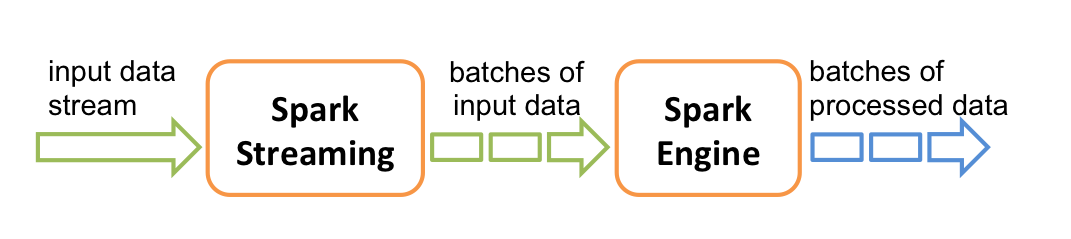
\includegraphics[width=0.8\textwidth]{includes/figures/fig_spark_layout}
  \caption{Illustration~\cite{Spark_doc_fig} depicting how Spark Streaming runs on-top of the Spark batch engine.}
  \label{fig:spark_stream_batch}
\end{figure}

This way of processing streams as a sequence of batches is all enabled through Spark Streaming's stream abstraction,
discretised streams, or DStreams. It differs to how streams are conceptualised in Samza and Storm in the way that while
streams are still, in essence, an unbounded sequence of data structures, being tuples in Storm, and message envelopes in
Samza, these data structures are the same data structure which is used to represented data batches in Spark. These are,
of course, the same resilient distributed dataset (RDD) data structure as explained in the previous chapter, in~\sectref{ssub:spark_streaming}.
Hence, Spark Streaming DStreams can be decomposed into a sequence of RDDs, making them fully compatible with batch-mode Spark~\cite{spark_stream_doc}.

For programming a Spark Streaming job, there are not a set of provided interfaces expected to be implemented, like in
Samza or Storm. Instead, all of the computations to be performed on streams are performed on an instantiation of the
\path{org.apache.spark.streaming.dstream.DStream} class returned from a DStream producing function from the
\path{org.apache.spark.streaming.StreamingContext} class~\cite{spark_stream_doc}. Processing performed on DStreams are generally programmed in
a dataflow fashion, with each function performed on the DStream returning a new DStream.

This way of operating on DStreams in a Spark Streaming program leads to all processing being contained in a single file,
whereas in Storm or Samza processing would be split between tasks or bolts written in different files. This leads to
more straightforward control over DStream transformations when programming, however also leads to much more tightly
coupled logic. This will be a topic of interest later when evaluating the different DSPS technologies.

\subsubsection{Input Component}

For the implementation of the input component design in Spark Streaming, Spark Streaming provides a native server socket input
system built-in on the \texttt{StreamingContext} class, available through the \texttt{socketTextStream} method. Hence
this has been used to open a connection on a particular server socket for inputting of speed data in the same manner as in the
Samza and Storm implementations.

\subsubsection{Processing Component}

For the implementation of the processing component design in Spark Streaming, a function has been written to test a single
speed value, testing whether or not it is between the specified speed limits. Depending on the outcome of the test,
a tuple is returned containing the original speed value, and a noise flag that is flagged if the data value is outside
of the speed limit.

This speed test function then gets mapped to the existing socket connection DStream, effectively running the function
for every speed value that is received over the connection.

\subsubsection{Output Component}

Unlike the Storm or Samza implementations, Spark Streaming offers no simple way to extend an existing streaming processing
project through means of extra processing tasks that operate on existing streams. However, it does afford extensibility
in the way of adding further processing on the DStream that is produced from previously performed operations, such
as the previously mentioned speed test function mapping.

\subsubsection{Deployment}

Spark Streaming programs are compiled and distributed in the same fashion in which Samza and Storm projects are. However,
for Spark Streaming programs written in Python using their relatively new PySpark API, compilation is unnecessary and an entire Spark
Streaming Python project can be distributed and submitted and run on different installations of Spark Streaming straight
from the Python source file. This greatly eases the distribution and deployment aspects of Spark Streaming, when using
PySpark, in relation to Storm topologies and Samza projects.

For our Spark Streaming pipeline implementation written in Scala, SBT\footnote{http://www.scala-sbt.org/} was used to assemble a JAR file containing compiled
bytecode, for ease of use over Maven with Scala projects. For the Spark Streaming pipeline implemented in Python, the
Python source files were simply used for deployment. Both methods enable the deployment of the Spark Streaming pipelines on
different Spark installations.

\textit{Note that the source code of our implementation can be seen in Appendix~\ref{lst:spark}.}

% subsubsection spark_streaming (end)




\section{Conclusion} % (fold)
\label{sub:implement_conclusion}

In conclusion this chapter has touched upon all details of implementation for each of the prototype pipelines.
We have detailed how each prototype data filtering pipeline has been built for each candidate system, ready
for subsequent tests and evaluation, of which will be discussed in the following chapter. Furthermore, the overall
design of the pipeline that has been implemented has been detailed along with the details of the overall testing
environment upon which the pipelines are to be implemented.

% subsection conclusion (end)